\section{Grid технология. Определение. Архитектура.}

\D{
    Grid вычисления - форма распределенных вычислений,
    представленная в виде кластеров, соединенных сетью
    слабосвязанных компьютеров, работающих вместе для выполнения
    огромного количества различных заданий.
}

Ядром Grid являются виртуальные организации и способы их взаимодействия.

Аспекты построения взаимодействий:
\begin{itemize}
    \item вычисления
    \item данные
    \item безопасность
\end{itemize}

\begin{figure}[h]
	\centering
	\begin{minipage}[b]{0.8\textwidth}
		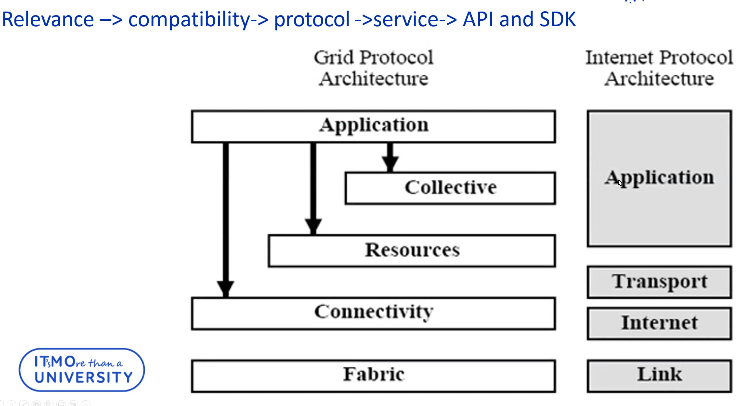
\includegraphics[width=\textwidth]{images/grid.png}
		\caption{GRID Архитектура}
	\end{minipage}
\end{figure}

Уровни
\begin{itemize}
    \item Fabric - уровень, позволяющий предоставить все ресурсы grid для более
    высокоуровневых взаимодействий. Под ресурсом понимаются: вычислительные
    ресурсы, ресурсы хранения, каталоги, сетевые ресурсы, сенсоры. Fabric унифицирует
    представление ресурса, реализуя все специфические особенности ресурса под единым
    интерфейсом взаимодействия. Основными категориями реализуемых методов
    являются запрос и управление.
    \begin{itemize}
        \item Запрос - предоставляет информацию и методы поддержки сервисных ресурсов
        \item Управление - основные методы управления ресурсом
        \item Globus Toolkit - базовый инструмент реализации
    \end{itemize}

    \item Connectivity - уровень, определяющий протоколы связи и аутентификации,
    необходимые для сети взаимодействия, специфичной для Grid, которые
    включают:
    \begin{itemize}
        \item Single-sign-on - одна точка входа;
        \item Делегирование - возможность запуска приложений с теми же правами,
        что и у пользователя;
        \item Интеграция - Kerberos и безопасность Unix;
        \item Доверительные отношения на основе пользователя - Если пользователь
        имеет права на ресурс А и ресурс B, то администраторам A и B не нужно
        взаимодействовать.
    \end{itemize}
    
    \item Ресурс - уровень, основанный на Connectivity и вызывающий методы Fabric,
    определяет протоколы (и API, и SDK), для безопасной связи, инициации, мониторинга,
    контроля, учета и оплаты отдельных операций обмена ресурсами.
    \begin{itemize}
        \item Информационные протоколы - используются для получения информации о структуре
        и состоянии
        ресурсов, таких как их конфигурация, текущая нагрузка и политика использования.
        \item Протоколы управления - используются для согласования доступа к общим ресурсам
        (включая предварительное бронирование и качество обслуживания) и для других
        операций, таких как - создание процесса или доступ к данным, мониторинг состояния
        операции и управление (например, завершение) самой выполненной операции.
    \end{itemize}

    \item Collective - уровни ресурсов, которые используются для групп ресурсов. Примеры:
    Служба каталогов, службы совместного
    размещения, планирования и посредничества, службы мониторинга и
    диагностики, службы репликации данных
\end{itemize}

\begin{figure}[h]
	\centering
	\begin{minipage}[b]{0.7\textwidth}
		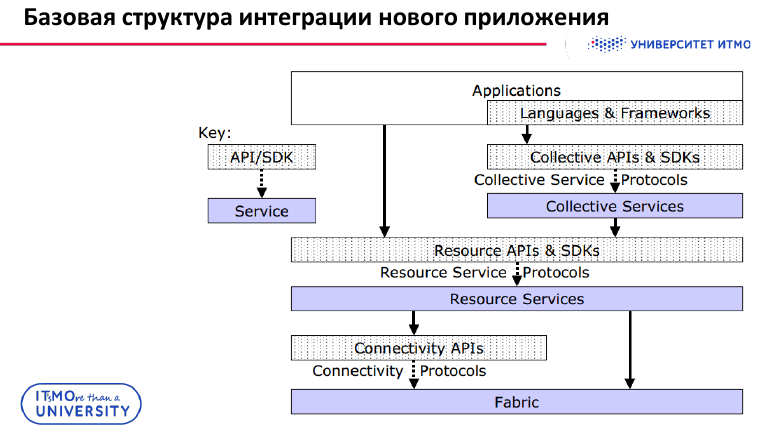
\includegraphics[width=\textwidth]{images/integr.png}
		\caption{GRID Интеграция приложений}
	\end{minipage}
\end{figure}